\section{Chiplet互联技术}

芯片能否成功跟上摩尔定律,很大程度上取决于芯片在一个封装中放置的距离,以确保它们之间快速、高带宽的电连接;就像单片 SoC 中的功能一样。Chiplet 互联技术是实现多 Die 系统(Multi-Die System)的关键,它定义了封装内不同芯片裸片(Die)之间如何进行高速、低延迟、高能效的数据通信。

3D 系统集成领域正在出现两个主要的行业方向:通过公共基板(也称为中介层)并排连接芯片的 2.5D 芯片集成和 3D-SoC,其中芯片彼此堆叠。Chiplets 提供了一个模块化系统,它将来自不同供应商和技术节点的独立芯片组合在一起,而不是将所有功能设计到一个单片系统中,下面将依次介绍不同的封装方式及与之对应的互联方式。

\subsection{2D MCM封装}

MCM(multi chip module, 多芯片组件) 封装, 即基板平面方向
集成多个芯片或芯粒, 是比较成熟的先进封装技术, 一般是指通过引
线键合 (bonding) 或/和倒装芯片 (flip chip) 技术实现芯粒和有机
基板 (substrate, 以下简称基板) 连通, 最终芯粒之间通过基板实现
互连。因为引线键合只能在芯粒四周出连线, 互连密度低, 信号线
长, 不利于高速信号互连, 所以在chiplet中更多应用基于高密度基板
的倒装芯片MCM, 基板上的走线宽度/间距可达$9/12\mu\text{m}$, 芯粒到芯
粒的间隙可以到 $1\text{ mm}$, 保证了芯粒互连信号质量, 同时有利于缩小
封装尺寸, 控制封装成本。采用MCM封装技术的典型芯片是AMD公
司基于Zen架构的服务器和台式电脑处理器芯片, 国内寒武纪公司云
端训练芯片思元$370$也采用MCM封装形式完成 $2$ 个芯粒的互连。

\subsection{2.3D封装}

2.3D 封装是指在一个有机转接板上实现芯粒之间的互连, 然后再 和基板相连, 如图 4(a) 所示。它将高密度有机转接板和低密度基板 分开制造, 便于提高基板良率和降低封装成本。 2.3D 封装中有机转接 板很薄, 由于没有玻纤等增强材料, 刚度很低, 所以翘曲 (warpage) 控制是个难点。

\begin{figure}[htbp]
	\centering
	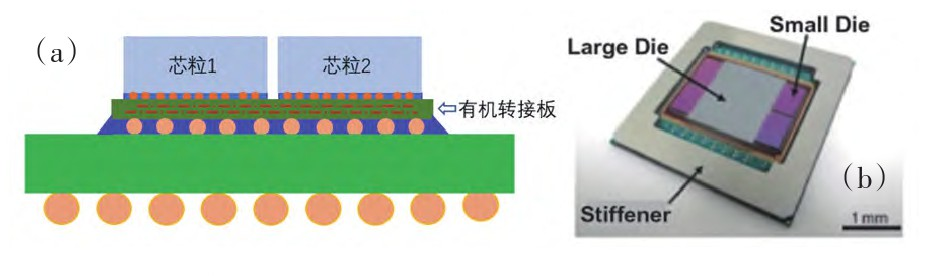
\includegraphics[width=0.6\textwidth]{img/3-2.jpg} % 图片文件名,不需要加扩展名
	\caption{$ \ 2.3\text{D}$ 封装概念图 $(\text{a})$ 及采用 $2.3\text{D}$ 封装的 $\text{Cisco}$ 公司芯片 $(\text{b})$ \cite{Miki2019Development}}
	\label{fig:example}
\end{figure}

目前有报道 Cisco 公司一款芯片已成功运用该技术, 产品线宽/间 距为 6/6μm, 集成 5 个芯粒, 如图 4(b) 
所示。国内目前已有公司 在开发双基板封装, 理念和 2.3D 封装类似, 只不过其基板互连密度没 有 2.3D 有机转接板高。

\subsection{2.5D中介层技术}
在 2.5D 集成中,芯片通过硅、有机聚合物、玻璃或层压板等公共基板连接。IMEC(Interuniversity Microelectronics Centre, 一家总部位于比利时鲁汶的独立研究机构)  目前专注于硅和有机基板的研究。虽然硅中介层是一种成熟的高性能应用技术,具有最精细的间距和良好的热电性能,但它们也具有更高的成本和复杂性。因此,有机基板作为替代方案正在被研究和优化。

早期的芯片集集成侧重于使用硅中介层基板实现芯片间的互连。这种集成需要将两个独立的芯片集非常紧密地(间距小于 50µm)放置在共用的中介层基板上,中介层基板上采用微米级布线来建立连接。硅中介层采用传统的 BEOL 铜/氧化物镶嵌工艺,以极高的良率实现微米和亚微米级互连间距。

IMEC提供的一种方案是硅“桥”,这是一种小型硅中介层,仅在边缘处将芯片连接在一起。
另一种替代方案是超细重分布层 (RDL) 互连技术,该技术用有机聚合物取代硅,并在其中嵌入一层铜线用于连接芯片。IMEC 目前正在优化这项技术,致力于达到与硅基互连技术类似的互连密度,并提高与硅基互连技术的兼容性。就间距而言,中介层仍然以亚微米间距占据主导地位;IMEC 的目标是将 RDL 间距提升至 2µm,甚至在未来实现亚微米级(图 5)。

\begin{figure}[htbp]
	\centering
	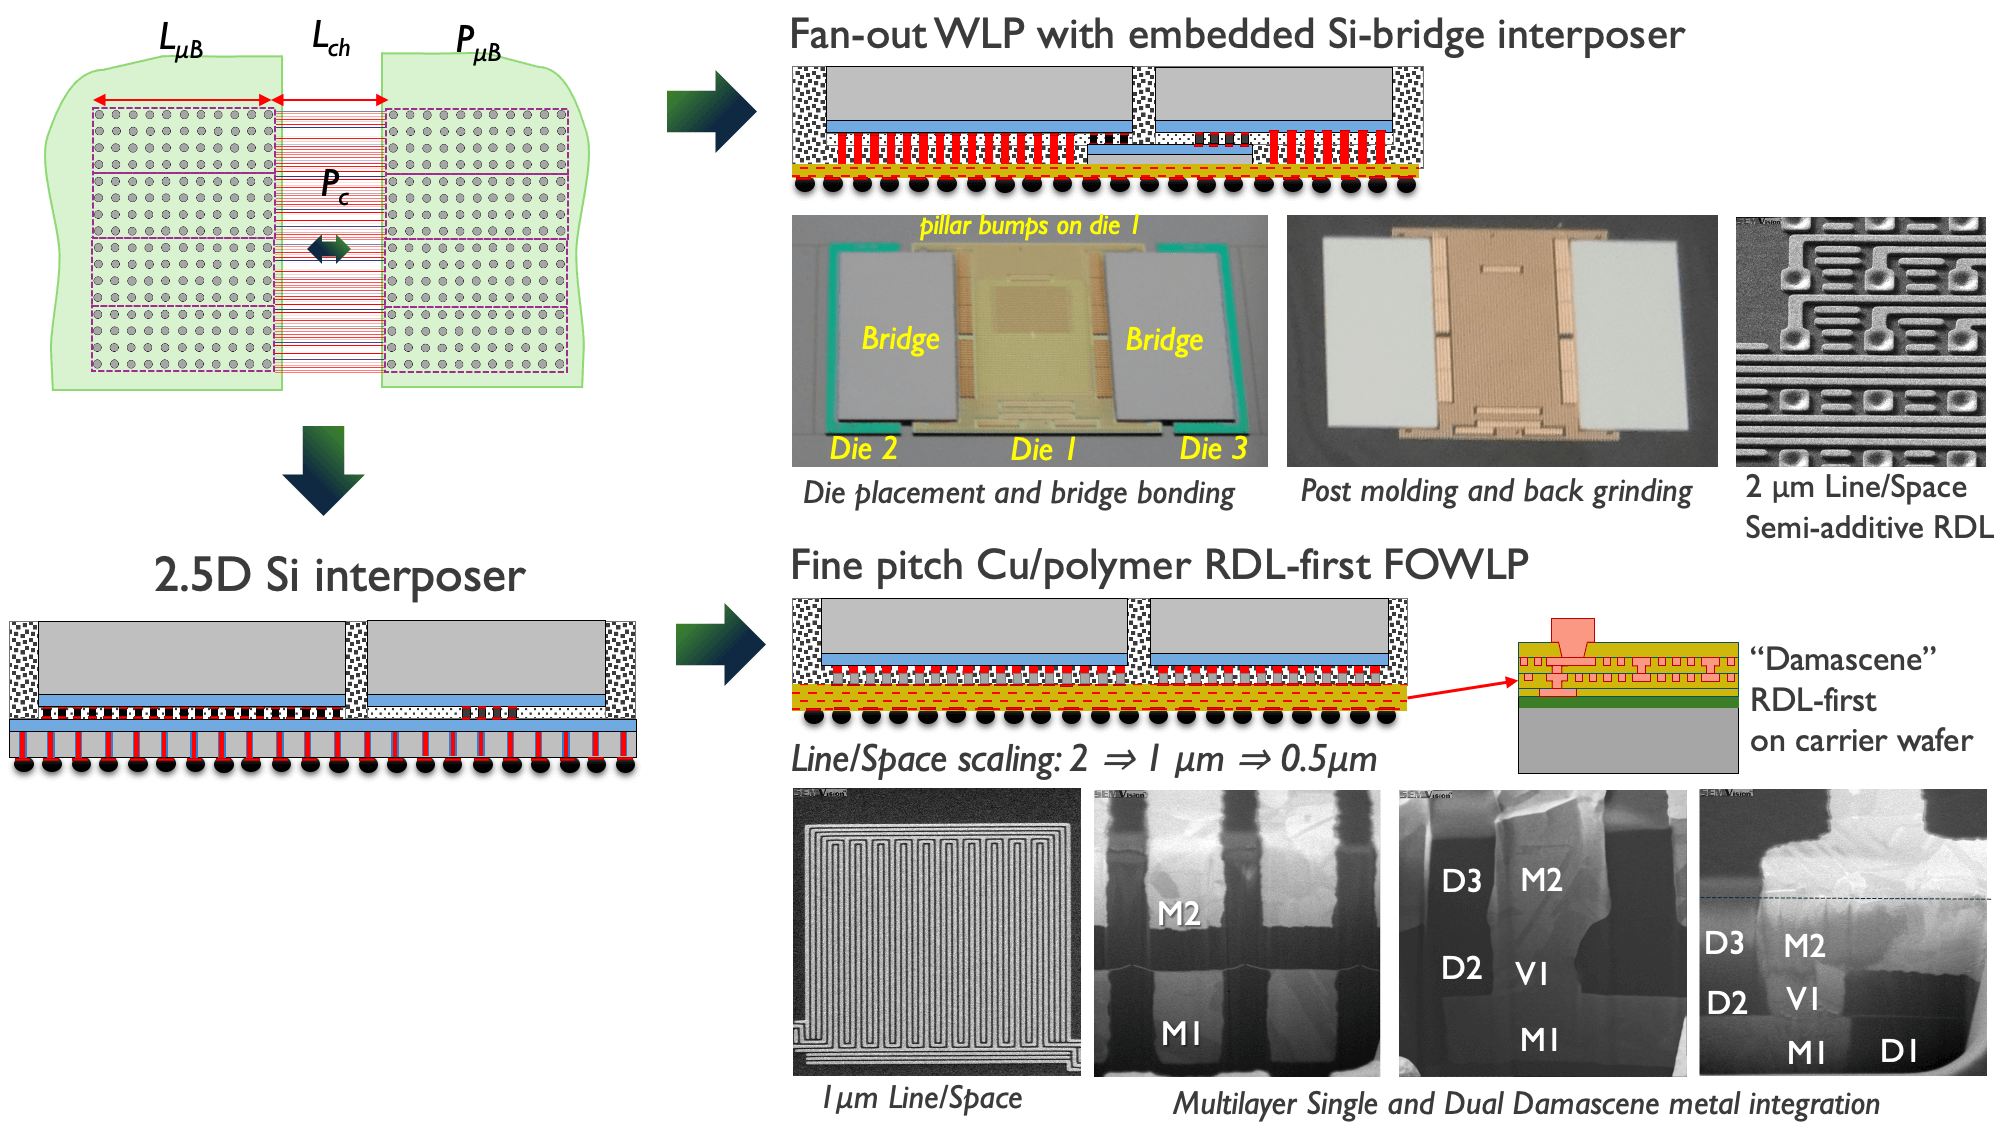
\includegraphics[width=0.8\textwidth]{img/2.-silicon-interposer-tech2.png} % 图片文件名,不需要加扩展名
	\caption{使用硅中介层进行集成的芯片集 \cite{Beyne2024Chiplet}}
	\label{fig:example}
\end{figure}

除了探索硅中介层技术的替代方案外,IMEC 还在研究如何通过添加额外功能,使中介层成为更有价值的组件。例如,中介层可以配备额外的去耦电容,以保护芯片免受噪声和电源异常的影响。

\subsection{3D片上系统:混合键合实现亚微米间距}

某些应用(例如高性能计算)可能需要高性能、更小的外形尺寸或更高的系统集成度,因此更倾向于采用完整的 3D 方法。无需建立横向连接,芯片集可以堆叠在一起,形成 3D-SoC \cite{8429741}。这种方法无需添加额外的模块,而是将芯片集进行协同设计,使它们像同一个芯片一样运行。

\begin{figure}[htbp]
	\centering
	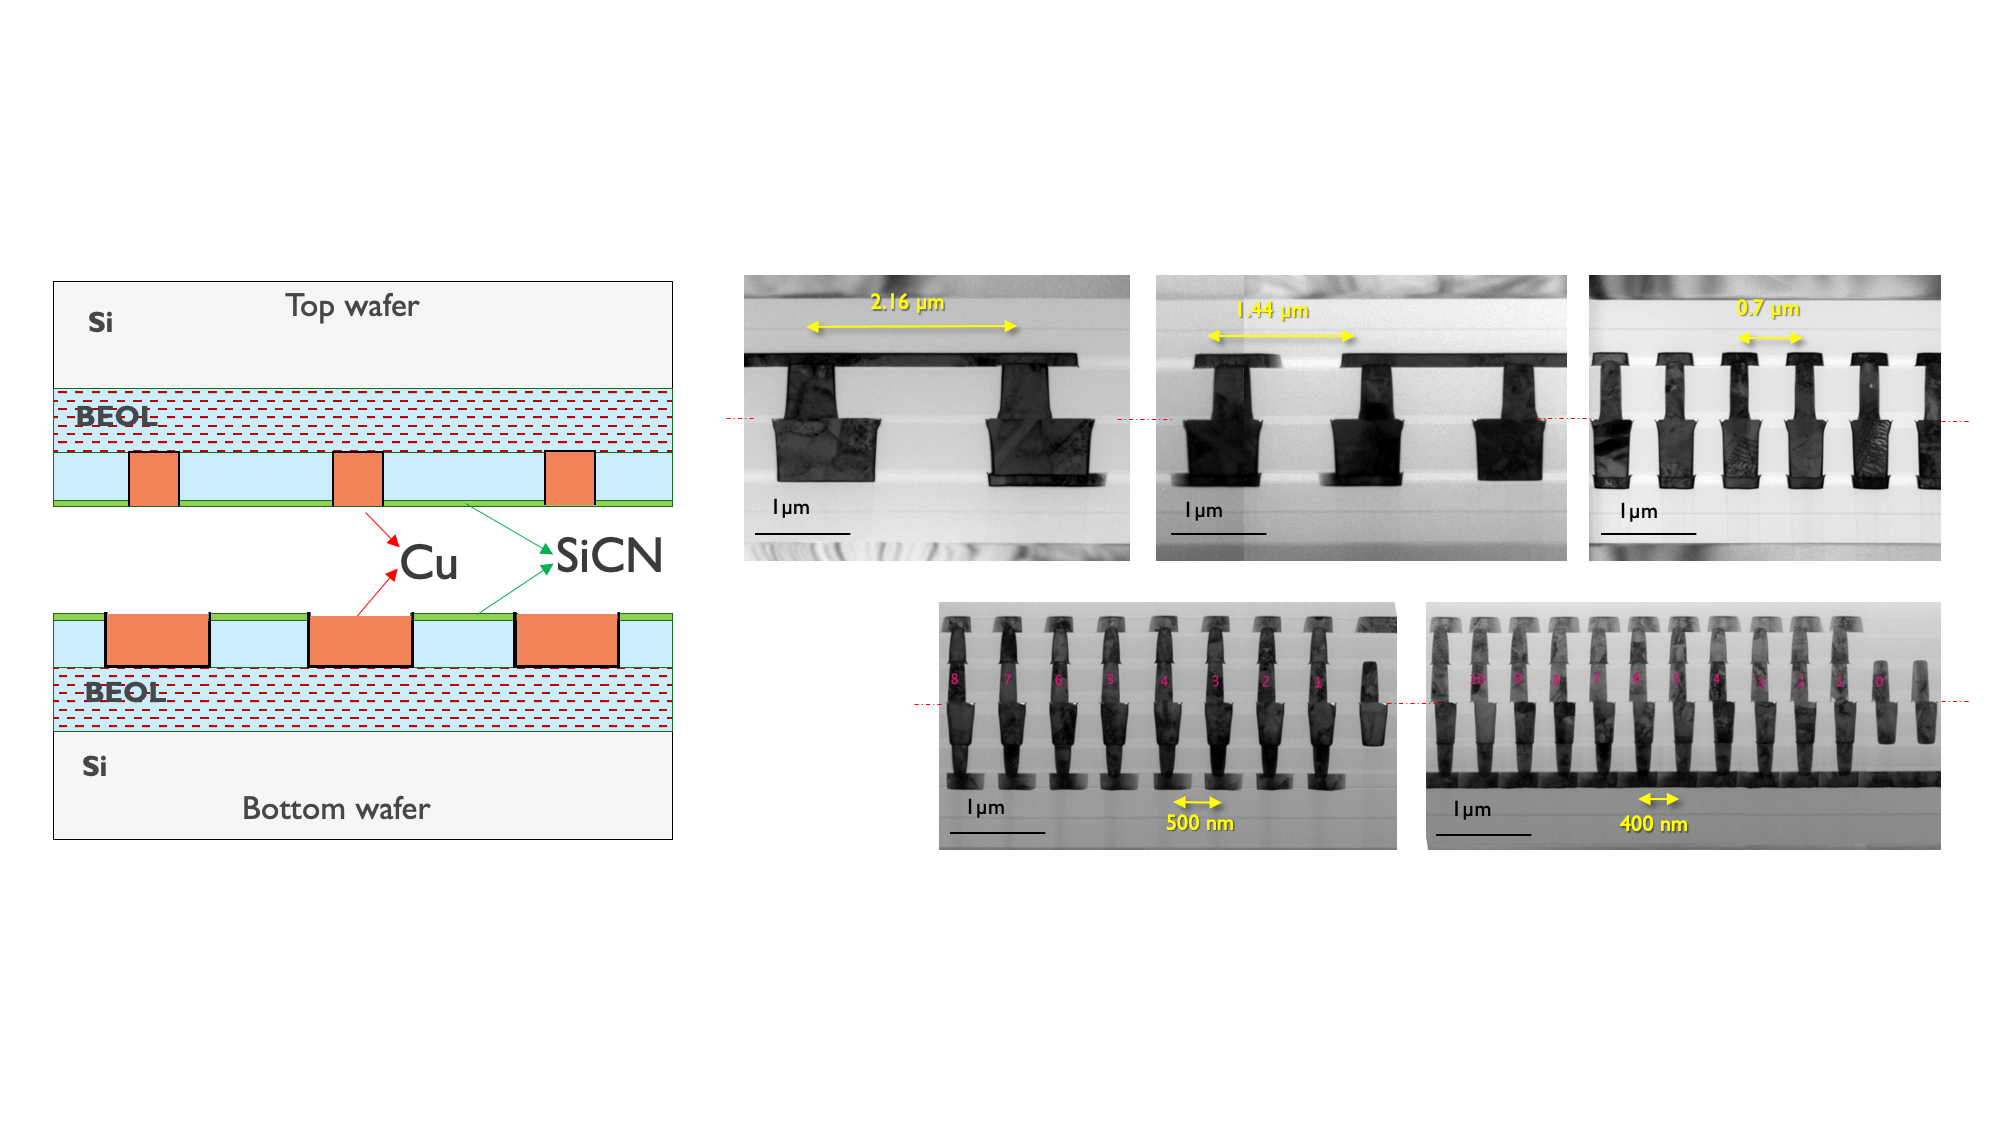
\includegraphics[width=0.8\textwidth]{img/3.-bump-pitch2.png} % 图片文件名,不需要加扩展名
	\caption{晶圆间混合键合(SiCN)用以实现微米级互连密度3D-SoC集成 }
	\label{fig:example}
\end{figure}

对于 2.5D 技术,芯片通过小型焊料凸块放置在中介层顶部,从而实现电气和机械连接。这些微凸块之间的间距越小,连接速度越快,稳定性也越高。工业界中微凸块的间距通常在 50µm 到 30µm 之间。

而晶圆间混合键合是实现微米级互连密度 3D-SoC 集成的关键技术。该技术将两个具有低温度膨胀系数的硅芯片连接在一起。该工艺的关键部件是电介质,它能够平坦化和激活堆叠层的表面,从而实现有效键合,并对堆叠中的不同芯片进行电绝缘。Imec 的专有方法采用 SiCN 作为键合电介质,将互连间距缩小至 700 纳米。其路线图甚至预测了 400 纳米和 200 纳米的间距(图 6)。


